\documentclass[12pt,aspectratio=169]{beamer}
\usetheme{metropolis}
\setbeamersize{text margin left=.5cm,text margin right=.5cm}
\usepackage[lf]{carlito}
\usepackage{siunitx}
\usepackage{tikz}
\usepackage{mathpazo}
\usepackage{bm}
\usepackage{mathtools}
\usepackage[ISO]{diffcoeff}
\diffdef{}{ op-symbol=\mathsf{d} }
\usepackage{xcolor,colortbl}

\setmonofont{Ubuntu Mono}
\setlength{\parskip}{0pt}
\renewcommand{\baselinestretch}{1}

\sisetup{
  inter-unit-product=\cdot,
  per-mode=symbol
}

\tikzset{
  >=latex
}

%\newcommand{\iii}{\hat{\bm\imath}}
%\newcommand{\jjj}{\hat{\bm\jmath}}
%\newcommand{\kkk}{\hat{\bm k}}

\usepackage{circuitikz} % to draw circuits!

\setlength{\parskip}{0pt}
\renewcommand{\baselinestretch}{1}

\sisetup{
  per-mode=symbol
}
\tikzset{
  >=latex,
  voltage dir=RP
}

\title{Topic 12: DC Circuit Analysis}
\subtitle{AP (1\&2) and IBHL Physics}
\author[TML]{Dr.\ Timothy Leung}
\institute{Olympiads School}
\date{Updated: Summer 2022}

\newcommand{\pic}[2]{
  \includegraphics[width=#1\textwidth]{#2}
}
\newcommand{\eq}[2]{
  \vspace{#1}{\Large
    \begin{displaymath}
      #2
    \end{displaymath}
  }
}
%\newcommand{\iii}{\ensuremath\hat{\bm{\imath}}}
%\newcommand{\jjj}{\ensuremath\hat{\bm{\jmath}}}
%\newcommand{\kkk}{\ensuremath\hat{\bm{k}}}
\newcommand{\iii}{\ensuremath\hat\imath}
\newcommand{\jjj}{\ensuremath\hat\jmath}
\newcommand{\kkk}{\ensuremath\hat k}



\begin{document}

\begin{frame}
  \maketitle
\end{frame}


\section{Circuits}

\begin{frame}{Basic DC Circuit}
  \begin{columns}
    \column{.3\textwidth}
    \centering
    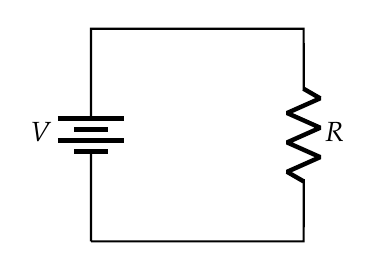
\begin{tikzpicture}[scale=1.8,american voltages]
      \draw[thick](0,0) to[battery,l=$V$]
      (0,1.5)--(1.5,1.5) to[R=$R$](1.5,0)--(0,0);
    \end{tikzpicture}
    
    \column{.7\textwidth}
    A basic circuits consists of:
    \begin{itemize}
    \item A voltage source: battery, generator or capacitor
    \item Connecting wires
    \item A load: resistors, motor, LEDs
    \end{itemize}
  \end{columns}
\end{frame}






\section{Current}

\begin{frame}{Current}
  The \textbf{electric current} $I$ through conductor is the amount of charge
  carriers $Q$ that passes through a point during a time interval $t$:

  \eq{-.2in}{
    \boxed{I=\frac{Q}t}
  }

  In general electric circuits, the current through a conductor is a function
  of time, and the $+/-$ signs may be used to indicate direction of the
  current.
\end{frame}



\begin{frame}{Current Through the Conductor}

  The expression for electric current can be expanded this way:
  
  \eq{-.15in}{
    I=\frac{Q}{t}=\left(\frac{Q}{V}\right)\frac{V}{t}
    =\left[ne\right]\left[Av_d\right]
  }
  where
  \begin{itemize}
  \item $Q/V$ is the \emph{amount of charges per volume}, which is also the
    \textbf{charge carrier density} (number of charge carriers per volume) $n$
    times the \textbf{elementary charge} $e$
  \item $V/t$ is the rate the volume of charges moves through the
    conductor, give by the cross-section area of the conductor $A$ times the
    \textbf{drift velocity} $v_d$ of the charge carrier
  \end{itemize}
%  For simplicity, we \emph{assume} that charge carriers are positive. While the
%  opposite is true, the behavior will be \emph{almost} identical.
\end{frame}



\begin{frame}{Current Through the Conductor}
  Combining the terms:

  \eq{-.2in}{
    \boxed{I=\frac Qt=neAv_d}
  }
  \begin{center}
    \begin{tabular}{l|c|c}
      \rowcolor{pink}
      \textbf{Quantity} & \textbf{Symbol} & \textbf{SI Unit} \\ \hline
      Current                               & $I$ & \si{\ampere} \\
      Charge carrier density                & $n$ & \si{\per\metre\cubed} \\
      Elementary charge                     & $e$ & \si{\coulomb}\\
      Cross-section area of the conductor   & $A$ & \si{\metre\squared}\\
      Drift velocity of the charge carriers & $v_d$ & \si{\metre\per\second}
    \end{tabular}
  \end{center}
  The calculation for the charge carrier density $n$ requires some additional
  thoughts.
\end{frame}



\begin{frame}{Charge Carrier Density}
  Calculating the charge carrier density in a \emph{metal} conductor involves
  some physical information about the metal:
  \begin{enumerate}
  \item Divide the metal's density $\rho$ by its molar mass $M$ to find the
    \emph{number of moles of atoms per unit volume}
  \item Multiply by Avogadro's number $N_A=\SI{6.0221e23}{\per mol}$ to find
    \emph{number of atoms per unit volume}
  \item Multiply by the number of free electrons per atom $k$ for that
    particular metal
  \end{enumerate}
\end{frame}



\begin{frame}{Charge Carrier Density}
  Collecting all the terms from the last slide, we have:
  
  \eq{-.15in}{
    \boxed{n=\frac{\rho kN_A}{M}}
  }
  \begin{center}
    \begin{tabular}{l|c|c}
      \rowcolor{pink}
      \textbf{Quantity} & \textbf{Symbol} & \textbf{SI Unit} \\ \hline
      Charge carrier density   & $n$    & \si{\per\metre\cubed} \\
      Density of material      & $\rho$ & \si{\kilo\gram\per\metre\cubed} \\
      Free electrons per atom  & $k$    & \\
      Avogadro's number        & $N_A$  & \si{\per\mol}\\
      Molar mass               & $M$    & \si{\kilo\gram\per\mol}
    \end{tabular}
  \end{center}
  For copper, $M=\SI{63.54e-3}{\kilo\gram\per\mol}$,
  $\rho=\SI{8.96e3}{\kilo\gram\per\metre\cubed}$, $k=1$ and therefore
  $n=\SI{8.5e28}{\per\metre\cubed}$.
\end{frame}


\begin{frame}{Current}
  Another alternate description of the electric current is to express it in
  terms of the current density $J$, with a unit of of \emph{amp\`{e}re per
    meters squared} (\si{\ampere\per\meter\squared}).

  \eq{-.2in}{
    \boxed{I=JA}
  }

  It is obvious from the previous expression that the current density is the
  product of the charge carrier density, elementary charge, and the drift
  velocity:

  \eq{-.2in}{
    \boxed{J=nev_d}
  }
\end{frame}


\begin{frame}{Conventional Current vs.\ Electron Flow}
  We have \emph{assumed} that the charge carriers are positively charged, which
  means that the current flows from high electric potential to low potential
  (i.e.\ from cathode to anode).
  \begin{center}
    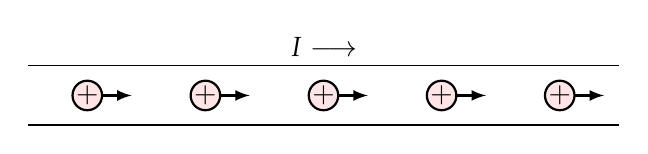
\begin{tikzpicture}[scale=.75]
      \draw (0,0)--(10,0);
      \draw (0,1)--(10,1) node[midway,above]{$I\longrightarrow$};
      \foreach \x in {1,3,...,9}{
        \draw[thick,fill=pink!40](\x,.5) circle(.25) node{$+$};
        \draw[thick,->](\x+.25,.5)--(\x+.75,.5);
      }
    \end{tikzpicture}
  \end{center}
  In a conducting wire, instead of positive charges flowing in one direction,
  we have, in fact, electrons (negative charges) flowing in the opposite
  direction, called the \textbf{electron current}:
  \begin{center}
    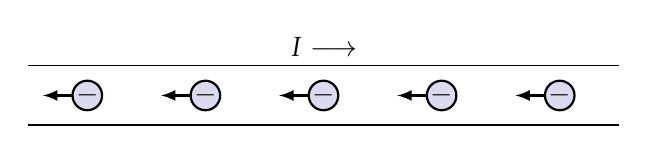
\begin{tikzpicture}[scale=.75]
      \draw (0,0)--(10,0);
      \draw (0,1)--(10,1) node[midway,above]{$I\longrightarrow$};
      \foreach \x in {1,3,...,9}{
        \draw[thick,fill=blue!40!gray!20](\x,.5) circle(.25) node{$-$};
        \draw[thick,->](\x-.25,.5)--(\x-.75,.5);
      }
    \end{tikzpicture}
  \end{center}
  For circuit analysis, we use the conventional current for simplicity.
%  \item We are treating current as a scalar quantity, but later we will have to
%    treat it as a vector
%  \item How much energy it loses depends on the resistance of the material
\end{frame}



\begin{frame}{Electric Field Inside the Wire}
  Inside the wire, there is a weak electric field, which exerts a force on the
  free electrons as they move in the wire
  \begin{itemize}
  \item As the charges move through a conductor, they lose potential energy
  \item Unlike a falling object which converts gravitational potential energy
    to kinetic energy, in a circuit, the energy is 
    \begin{itemize}
    \item converted into radiative heat or light through the resistance of the
      wire, or
    \item converted into kinetic energy of a motor shaft
    \end{itemize}
  \end{itemize}
\end{frame}



\section{Resistors}

\begin{frame}{Resistance of a Conductor}
  The resistance of a conductor is proportional to the resistivity $\rho$ and
  its length $L$, and inversely proportional to the cross-sectional area $A$:

  \eq{-.2in}{
    \boxed{R = \rho\frac{L}{A}}
  }
  \begin{center}
    \begin{tabular}{l|c|c}
      \rowcolor{pink}
      \textbf{Quantity} & \textbf{Symbol} & \textbf{SI Unit} \\ \hline
      Resistance           & $R$    & \si{\ohm} \\
      Resistivity          & $\rho$ & \si{\ohm.\metre}\\
      Length of conductor  & $L$    & \si{\metre}\\
      Cross-sectional area & $A$    & \si{\metre\squared}
    \end{tabular}
  \end{center}
  The resistivity $\rho$ is determined by the material.
\end{frame}


\begin{frame}{Resistivity}
  The resistivity of a material is the ratio between strength of the electric
  field $E$ inside the material and the current density $J$:

  \eq{-.2in}{
    \boxed{\rho=\frac{E}J}
  }
  \begin{itemize}
  \item Conductor: the electrons are free to move, therefore the electric
    field tend to be very small, and the resistivity is low.
  \item Insulators and dielectric: electrons cannot move easily (dielectric:
    they can only polarize themselves) the electric field are generally
    strong, and the resistivity is higher.
  \end{itemize}
\end{frame}



\begin{frame}{Resistance of a Conductor}
  \eq{-.01in}{
    \boxed{R=\rho\frac{L}A}
  }

  \begin{columns}
    \column{.5\textwidth}
    \begin{center}
      \begin{tabular}{c|c|c}
        \rowcolor{blue!50}
        {\color{white}Gauge} & 
        {\color{white}Diameter} & 
        {\color{white}$R/L$} \\
        \rowcolor{blue!50}
        & {\color{white}(\si{mm})} & 
        {\color{white}(\SI{e-3}{\ohm\per\metre})}\\ \hline
        0  & \num{9.35} & \num{0.31} \\
        10 & \num{2.59} & \num{2.20} \\
        14 & \num{1.63} & \num{8.54} \\
        18 & \num{1.02} & \num{21.90} \\
        22 & \num{0.64} & \num{51.70} \\
      \end{tabular}
    \end{center}
    
    \column{.5\textwidth}
    \begin{center}
      \begin{tabular}{c|c}
        \rowcolor{blue!50}
        {\color{white} Material} & 
        {\color{white} Resistivity $\rho$ (\si{\ohm\metre})}\\ \hline
        silver    & \num{1.6e-8} \\
        copper    & \num{1.7e-8} \\
        aluminum  & \num{2.7e-8} \\
        tungsten  & \num{5.6e-8} \\
        Nichrome  & \num{100e-8} \\
        carbon    & \num{3500e-8}\\
        germanium & \num{.46} \\
        glass     & \num{e10} to \num{e14}\\
      \end{tabular}
    \end{center}
  \end{columns}
\end{frame}



\section{Ohm's Law}

\begin{frame}{Ohm's Law}
  The electric potential difference $V$ across a resistor equals the product of
  the current $I$ through the load and the resistance $R$:

  \eq{-.2in}{
    \boxed{V=IR}
  }
  \begin{center}
    \begin{tabular}{l|c|c}
      \rowcolor{pink}
      \textbf{Quantity} & \textbf{Symbol} & \textbf{SI Unit} \\ \hline
      Potential difference & $V$    & \si{\volt} \\
      Current              & $I$    & \si{\ampere}\\
      Resistance           & $R$    & \si{\ohm}
    \end{tabular}
  \end{center}
  A resistor is considered ``ohmic'' if it obeys Ohm's law. Note that Ohm's law
  is not a fundamental law in physics.
\end{frame}


\begin{frame}{Power Dissipated by a Resistor}
  Average power $P$ is the rate at which work $W$ is done, and from
  electrostatics, the change in electric potential energy $\Delta E_q$ (i.e.\
  the work done!) is proportional to the amount of charge $q$ and the voltage
  $V$. This gives a very simple expression for power through a resistor:
  
  \eq{-.15in}{
    P
    =\frac{W}{\Delta t}=\frac{\Delta (qV)}{\Delta t}
    =\left(\frac{\Delta q}{\Delta t}\right)V
    \;\rightarrow\;\boxed{P=IV}
  }
  \begin{center}
    \begin{tabular}{l|c|c}
      \rowcolor{pink}
      \textbf{Quantity} & \textbf{Symbol} & \textbf{SI Unit} \\ \hline
      Power through a resistor    & $P$ & \si{\watt} \\
      Current through a resistor  & $I$ & \si{\ampere} \\
      Voltage across the resistor & $V$ & \si{\volt}
    \end{tabular}
  \end{center}
\end{frame}



\begin{frame}{Other Equations for Power}
  When we combine Ohm's law ($V=IR$) with power equation, we get two additional
  expressions for power through a resistor:

  \eq{-.15in}{
    \boxed{P=\frac{V^2}R}\quad\boxed{P=I^2R}
  }
  \begin{center}
    \begin{tabular}{l|c|c}
      \rowcolor{pink}
      \textbf{Quantity} & \textbf{Symbol} & \textbf{SI Unit} \\ \hline
      Power      & $P$ & \si{\watt} \\
      Voltage    & $V$ & \si{\volt} \\
      Resistance & $R$ & \si{\ohm}  \\
      Current    & $I$ & \si{\ampere}
    \end{tabular}
  \end{center}
  Not surprisingly, these equations will only apply to ohmic devices.
\end{frame}


\section{Kirchhoff's Laws}

\begin{frame}{Current Law}
  The electric current that flows into any junction in an electric circuit must
  be equal to the current which flows out.

  \vspace{.2in}
  \begin{columns}
    \column{.3\textwidth}
    \begin{center}
      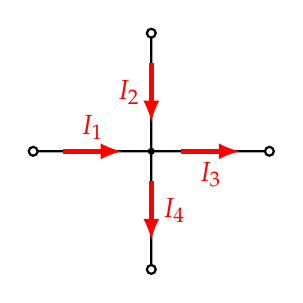
\begin{tikzpicture}[scale=1.5]
        \draw[thick](0,0) to[short,o-] (1,0) to[short,-o] (1,-1);
        \draw[thick](1,1) to[short,o-] (1,0) to[short,-o] (2,0);
        \draw[ultra thick,red,->](.25,0)--(.75,0) node[midway,above]{$I_1$};
        \draw[ultra thick,red,->](1,.75)--(1,.25) node[midway,left]{$I_2$};
        \draw[ultra thick,red,->](1.25,0)--(1.75,0) node[midway,below]{$I_3$};
        \draw[ultra thick,red,->](1,-.25)--(1,-.75) node[midway,right]{$I_4$};
        \fill[black](1,0) circle(0.03);
      \end{tikzpicture}
    \end{center}
    
    \column{.7\textwidth}
    e.g.\ if there are 4 paths to the junction at the center, with $I_1$ and
    $I_2$ going into the junction, and $I_3$ and $I_4$ coming out, then the
    current law says that

    \eq{-.3in}{
      I_1+I_2-I_3-I_4=0
    }
  \end{columns}

  \vspace{.2in}Basically, it means that there cannot be any accumulation of
  charges anywhere in the circuit. The law is a consequence of conservation of
  energy.
\end{frame}



\begin{frame}{Voltage Law}
  The voltage changes around any closed loop in the circuit must sum to zero,
  no matter what path you take through an electric circuit.

  \vspace{.1in}
  \begin{columns}
    \column{.3\textwidth}
    \begin{center}
      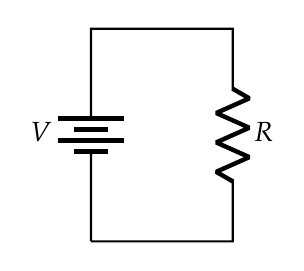
\begin{tikzpicture}[scale=1.8,american voltages]
        \draw[thick](0,0) to[battery,l=$V$] (0,1.5)--(1,1.5)
        to[R=$R$] (1,0)--(0,0);
      \end{tikzpicture}
    \end{center}
    \column{.7\textwidth}
    Assume that the current flows clockwise and we draw a clockwise loop, we
    get

    \eq{-.2in}{ V-V_R=0\;\;\rightarrow\;\; V-IR=0}

    \vspace{-.25in}If I incorrectly guess that $I$ flows counterclockwise, I
    will still have a similar expression

    \eq{-.25in}{-V_R-V=0\;\;\rightarrow\;\; -V-IR=0}
  \end{columns}

  \vspace{-.1in}When solving for $I$, we get a negative number, indicating
  that my guess was in the wrong direction.
\end{frame}



\section{Resistors in Circuits}

\begin{frame}{Resistors in Parallel}
  \begin{columns}
    \column{.32\textwidth}
    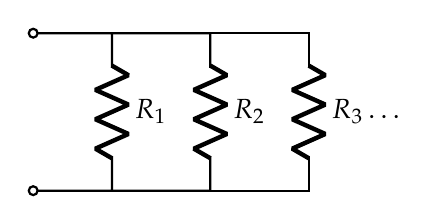
\begin{tikzpicture}
     \draw[thick](0,2)  to[short,o-] (1,2)to[R=$R_1$] (1,0) to[short,-o] (0,0);
     \draw[thick](1,2)  to[short] (2.25,2)to[R=$R_2$] (2.25,0)to[short] (1,0);
     \draw[thick](2.25,2)to[short](3.5,2) to[R=$R_3\ldots$] (3.5,0)
     to[short] (2.25,0);
    \end{tikzpicture}
    
    \column{.68\textwidth}
    From the current law, we know that the total current is the
    current through all the resistors, which we can rewrite in terms of voltage
    and resistance using Ohm's law:

    \eq{-.3in}{
      I=I_1+I_2+I_3\cdots=\frac{V_1}{R_1}+\frac{V_2}{R_2}+\frac{V_3}{R_3}\cdots
    }
    
    \vspace{-.1in}But since we also know that $V_1=V_2=V_3=\cdots=V$ from the
    voltage law, we can re-write as

    \eq{-.3in}{
      I=\frac{V}{R_p}=V\left(\frac1{R_1}+\frac1{R_2}+\frac1{R_3}\cdots\right)
    }
  \end{columns}
\end{frame}



\begin{frame}{Equivalent Resistance in Parallel}
  Applying applying Ohm's law and Kirchhoff's laws gives the equivalent
  resistance of a parallel circuit: the inverse of the equivalent resistance
  for resistors connected in parallel is the sum of the inverses of the
  individual resistances.

  \eq{-.2in}{
    \boxed{
      \frac1{R_p}=\sum_i^N\frac1{R_i}
    }
  }
  \begin{center}
    \begin{tabular}{l|c|c}
      \rowcolor{pink}
      \textbf{Quantity} & \textbf{Symbol} & \textbf{SI Unit} \\ \hline
      Equivalent resistance in parallel & $R_p$ & \si{\ohm} \\
      Resistance of individual loads    & $R_{1,2,3,\cdots,N}$ & \si{\ohm}
    \end{tabular}
  \end{center}
\end{frame}



\begin{frame}{Resistors in Series}
  \begin{center}
    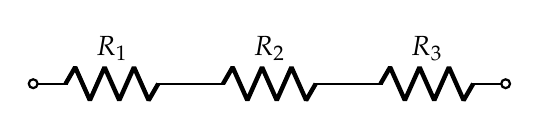
\begin{tikzpicture}
      \draw[thick](0,0) to[R=$R_1$,o-] (2,0) to[R=$R_2$] (4,0)
      to[R=$R_3$,-o] (6,0);
    \end{tikzpicture}
  \end{center}

  \vspace{.1in}The analysis for resistors in series is similar (but easier).
  From the current law, the current through each resistor is the same:

  \eq{-.2in}{
    I_1=I_2=I_3=\cdots=I
  }

  \vspace{-.1in}And the total voltage drop across all resistor is therefore:

  \eq{-.2in}{
    V=V_1+V_2+V_3+\cdots=I(\underbrace{R_1+R_2+R_3+\cdots}_{R_s})
  }
\end{frame}



\begin{frame}{Equivalent Resistance in Series}
  Again, through applying Ohm's law and Kirchhoff's laws, we find that when
  resistors are connected in series: the equivalent resistance of loads is the
  sum of the resistances of the individual loads.
  
  \eq{-.2in}{
    \boxed{R_s=\sum_{i=1}^{N}R_i}
  }
  \begin{center}
    \begin{tabular}{l|c|c}
      \rowcolor{pink}
      \textbf{Quantity} & \textbf{Symbol} & \textbf{SI Unit} \\ \hline
      Equivalent resistance in series & $R_s$ & \si{\ohm} \\
      Resistance of individual loads & $R_{1,2,3,\cdots,N}$ & \si{\ohm}
    \end{tabular}
  \end{center}
\end{frame}



\begin{frame}{Tips for Solving ``Simple'' Circuit Problems}
  \begin{enumerate}
  \item Identify groups of resistors that are in parallel or in series, and
    find their equivalent resistance.
  \item Gradually reduce the entire circuit to one voltage source and one
    resistor.
  \item Using Ohm's law, find the current out of the battery.
  \item Using Kirchhoff's laws, find the current through each of the resistors.
  \end{enumerate}
\end{frame}



\begin{frame}{Multi-Loop Circuits}
  \begin{columns}
    \column{.43\textwidth}
    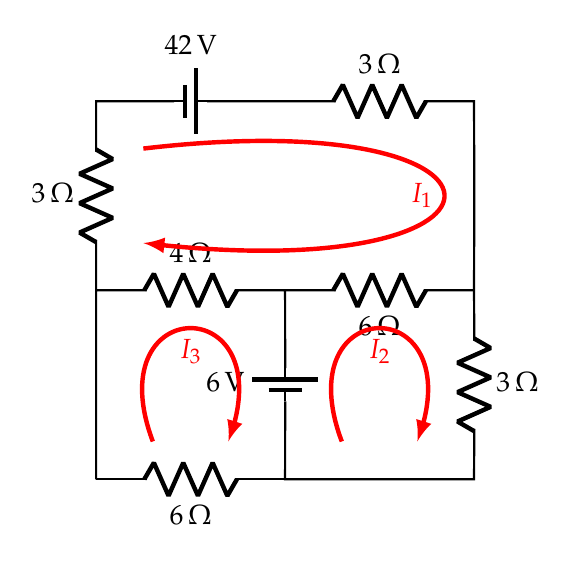
\begin{tikzpicture}[american voltages,scale=1.2]
      \draw[thick](0,0) to[short](0,2)
      to[R=\SI{3}{\ohm}] (0,4)
      to[battery1,l=\SI{42}{\volt}](2,4)
      to[R=\SI{3}{\ohm}](4,4) to[short](4,2)
      to[R=\SI{3}{\ohm}](4,0) to[short](2,0)
      to[battery1,l=\SI{6}{\volt}](2,2)
      to[R,l_=\SI{4}{\ohm}](0,2);
      \draw[thick](0,0) to[R,l_=\SI{6}{\ohm}](2,0);
      \draw[thick](2,2) to[R,l_=\SI{6}{\ohm}](4,2);
      \uncover<2->{
        \draw[ultra thick,red,->]
        (.5,3.5)..controls(4.75,4)and(4.75,2)..(.5,2.5)
        node[midway,left]{$I_1$};
        \draw[ultra thick,red,->] (0.6,0.4)..controls (0,2) and (2,2)..(1.4,.4)
        node[midway,below]{$I_3$};
        \draw[ultra thick,red,->] (2.6,0.4)..controls (2,2) and (4,2)..(3.4,.4)
        node[midway,below]{$I_2$};
      }
    \end{tikzpicture}
   
    \column{.57\textwidth}
    \begin{itemize}
    \item To solve this problem, we define a few `` current loops'' around the
      circuit: one on top, one on bottom left, and one on bottom right.
    \item<2-> Apply the voltage law in the loops. For example, in the
      lower left:

      \eq{-.5in}{
        4(I_1-I_3)-6-6I_3=0
      }      
    \item<2->\vspace{-.1in} Solve the system of equations to find the current.
      If the current that you worked out is negative, it means that you have the
      direction wrong.
    \end{itemize}
  \end{columns}
\end{frame}



\section{Capacitors in Circuit}

\begin{frame}{Capacitors in Parallel}
  \begin{center}
    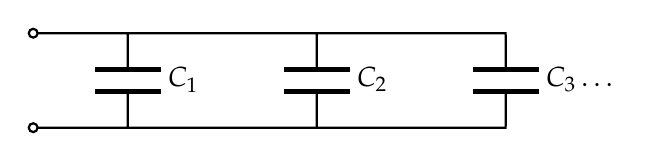
\begin{tikzpicture}[scale=1.2]
      \draw[thick](0,1)to[short,o-](1,1) to[C=$C_1$] (1,0)to[short,-o](0,0);
      \draw[thick](1,1)--(3,1) to[C=$C_2$]       (3,0)--(1,0);
      \draw[thick](3,1)--(5,1) to[C=$C_3\ldots$] (5,0)--(3,0);
    \end{tikzpicture}
  \end{center}
  From the voltage law, we know that the voltage across all the capacitors are
  the same, i.e.\ $V_1=V_2=V_3=\cdots=V$. We can express the total charge
  $Q_{tot}$ stored across all the capacitors in terms
  of capacitance and this
  common voltage $V$: 

  \eq{-.3in}{
    Q_{tot}=Q_1+Q_2+Q_3+\cdots=C_1V+C_2V+C_3V+\cdots
  }
  
  \vspace{-.1in}Factoring out $V$ from each term gives us the equivalent
  capacitance:

  \eq{-.2in}{
    \boxed{C_p=\sum_i C_i}
  }
\end{frame}


\begin{frame}{Capacitors in Series}
  Likewise, we can do a similar analysis to capacitors connected in series.
  \begin{center}
    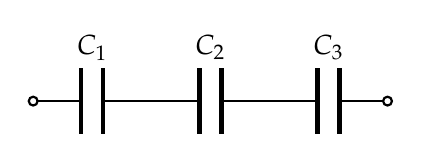
\begin{tikzpicture}[scale=1.2]
      \draw[thick](0,0) to[C=$C_1$,o-] (1.25,0) to[C=$C_2$] (2.5,0)
      to[C=$C_3$,-o] (3.75,0);
    \end{tikzpicture}
  \end{center}
  The total voltage across these capacitors are the sum of the voltages across
  each of them, i.e.\ $V_{tot}=V_1+V_2+V_3+\cdots$
  
  \vspace{.1in}We recognize that the charge stored on all the capacitors must
  be the same! We can then write the total voltage in terms of capacitance and
  charge:

  \eq{-.25in}{
    V_{tot}=\frac{Q}{C_1}+\frac{Q}{C_2}+\frac{Q}{C_3}+\cdots
  }
\end{frame}




\begin{frame}{Capacitors in Series}{Equivalent Capacitance}
  The inverse of the equivalent capacitance for $N$ capacitors connected in
  series is the sum of the inverses of the individual capacitance.

  \eq{-.2in}{
    \boxed{ \frac1{C_s}=\sum_i\frac1{C_i} }
  }
  
  Make sure we don't confuse ourselves with resistors.
\end{frame}



\begin{frame}{How Do We Know That Charges Are The Same?}
  It's simple to show that the charges across all the capacitors are the same
  \begin{center}
    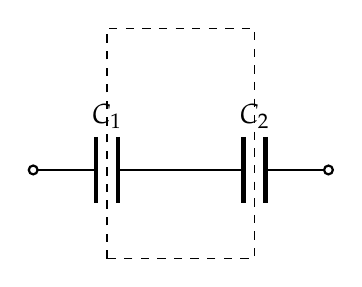
\begin{tikzpicture}[scale=1.5]
      \draw[thick](0,0) to[C=$C_1$,o-] (1.25,0) to[C=$C_2$,-o] (2.5,0);
      \draw[dashed](0.625,-.75) rectangle (1.875,1.2);
    \end{tikzpicture}
  \end{center}
  The capacitor plates and the wire connecting them are really one piece of
  conductor. There is nowhere for the charges to leave the conductor, therefore
  when charges are accumulating on $C_1$, $C_2$ must also have the same charge
  because of conservation of charges.
\end{frame}



\section{R-C Circuits}

\begin{frame}{Circuits with Resistors and Capacitors}
  Now that we have seen how resistors and capacitors behave in a circuit, we
  can look into combining them in to an ``R-C circuit''.
  \begin{center}
    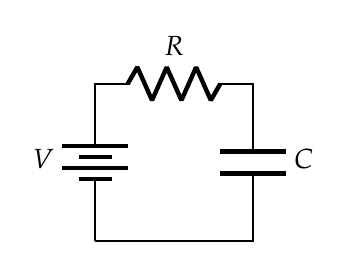
\begin{tikzpicture}[american voltages]
      \draw[thick](0,0) to[battery,l=$V$] (0,2) to[R=$R$] (2,2)
      to[C=$C$] (2,0)--(0,0);
    \end{tikzpicture}
  \end{center}
  The simplest form is a resistor and capacitor connected in series, and
  then connect to a voltage source. Because of the nature of capacitors, the
  current through the circuit will not be steady as were the case with only
  resistors.
\end{frame}



\begin{frame}{Discharging a Capacitor}
  The expression of charge across the capacitor is time-dependent:

  \eq{-.15in}{\boxed{Q(t)=Q_0e^{-t/\tau}}}

  \vspace{-.1in}where $Q_0=Q_{tot}$ is the initial charge on the
  capacitor, and $\tau=RC$ is called the \textbf{time constant}. Using a bit of
  basic calculus gives the current through the circuit:

  \eq{-.15in}{
    \boxed{I(t)=I_0e^{-t/\tau}}
  }

  where the initially current is given by
  $\displaystyle I_0=I(0)=\frac{Q_{tot}}{\tau}$.
\end{frame}



\begin{frame}{Charging a Capacitor}
  When charging the capacitor, the charge across the capacitor is given by:
  
  \eq{-.22in}{
    \boxed{Q(t)=Q_{tot}(1-e^{-t/RC})}
  }

  \vspace{-.1in}the time constant $\tau=RC$ is the same as the discharging case

  \vspace{.1in}\begin{columns}
    \column{.27\textwidth}
    \vspace{-.25in}
    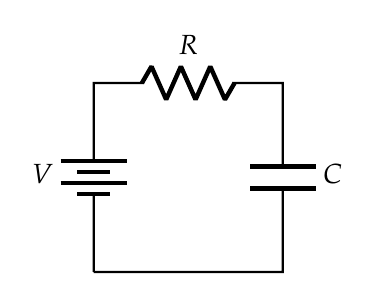
\begin{tikzpicture}[american voltages,scale=1.2]
      \draw[thick](0,0)
      to[battery,l=$V$] (0,2)
      to[R=$R$] (2,2)
      to[C=$C$] (2,0)--(0,0);
    \end{tikzpicture}
    
    \column{.73\textwidth}
    The current $I$ through the circuit is the same as the discharging case:
    
    \eq{-.22in}{
      \boxed{I_c(t)=I_0e^{-t/\tau}}
    }

    The initial current $I_0=Q_{tot}/\tau=V/R$. This makes sense because
    $V_C=0$ at $t=0$, and all of the energy must be dissipated through the
    resistor. At $t=\infty$, current through the capacitor is $I_c=0$
  \end{columns}
\end{frame}



\begin{frame}{Two Small Notes}
  \begin{enumerate}
  \item When a capacitor is uncharged, there is no voltage across the plate,
    it acts like a short circuit.
  \item When a capacitor is charged, there is a voltage across it, but no
    current flows \emph{through} it. Effectively it acts like an open circuit.
  \end{enumerate}
\end{frame}



\begin{frame}{A Slightly More Difficult Problem}
  \begin{center}
    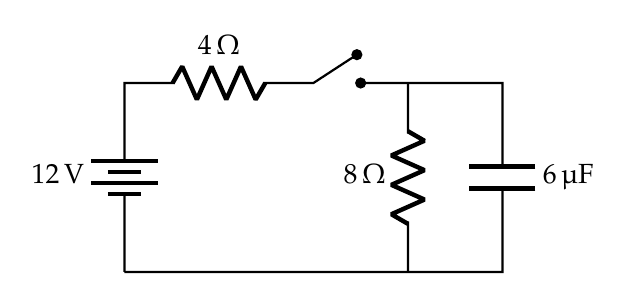
\begin{tikzpicture}[scale=1.2,american voltages]
      \draw[thick] (0,0)
      to[battery,l=\SI{12}{\volt}] (0,2)
      to[R=\SI{4}{\ohm}](2,2)
      to[short,-*](2.46,2.3);
      \draw[thick](2.5,2) to[short,*-] (3,2) to[short] (4,2)
      to[C=\SI{6}{\micro\farad}] (4,0)--(0,0);
      \draw[thick] (3,0) to[R=\SI{8}{\ohm}] (3,2);
    \end{tikzpicture}
  \end{center}
  \textbf{Example:} The capacitor in the circuit is initially uncharged. Find
  the current through the battery
  \begin{enumerate}
  \item Immediately after the switch is closed
  \item A long time after the switch is closed
  \end{enumerate}
\end{frame}
\end{document}
